\section{Experiment 1.2}

In order to eliminate some of these potential problems during
experiment 1 and 1.1, resulting in the outliers, the next attempt was
made using a separate computer acting as a USB host for the audio
device. This host used the Arch based operating system Manjaro.

Figure \ref{fig:experiment-1-2} shows the result of using this
separate host for the audio communication, and the previous host only
for the programmer and the logic analyzer. Now the outliers are all
gone, and left is a rate of about two milliseconds with a very minor
deviation. The packet sizes are still all 288 bytes long.

\begin{figure}[h]
	\caption{Rate over time and buffer length over time respectively
	for experiment 1.2}
	\centering
	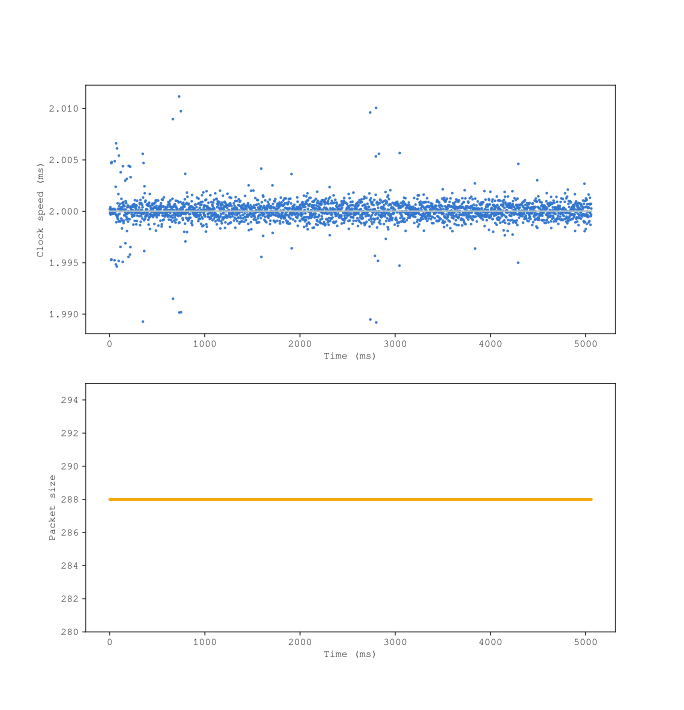
\includegraphics[width=0.8\textwidth]{Experiment-1/Experiment-1-2.png}
	\label{fig:experiment-1-2}
\end{figure}

The experiments 1, 1.1 and 1.2 shows that a rate of USB packets and
the size of the data contained in them can be measured. This is
measured with a low deviation in time, meaning that any change in rate
would be easily observed.

The next step is to try to make a request to the audio host for a
higher audio rate. The goal is to measure the size of each packet
increasing, as the host increases this rate.
